\documentclass[10pt,a4paper]{article}
\usepackage[utf8]{inputenc}

\usepackage{amsmath}
\usepackage{amsfonts}
\usepackage{amssymb}
\usepackage{graphicx}
\usepackage{listings}
\usepackage[margin=1.0in]{geometry}
\usepackage{caption}
\usepackage{subcaption}
\usepackage{float}
\usepackage[utf8]{inputenc}
\usepackage{refstyle}


\lstset{numbers=left,
	title=\lstname,
	numberstyle=\tiny, 
	breaklines=true,
	tabsize=4,
	language=Python,
	morekeywords={with,super,as},,
	frame=single,
	basicstyle=\footnotesize\tt,
	commentstyle=\color{comment},
	keywordstyle=\color{keyword},
	stringstyle=\color{string},
	backgroundcolor=\color{background},
	showstringspaces=false,
	numbers=left,
	numbersep=5pt,
	literate=
		{æ}{{\ae}}1
		{å}{{\aa}}1
		{ø}{{\o}}1
		{Æ}{{\AE}}1
		{Å}{{\AA}}1
		{Ø}{{\O}}1
	}
\usepackage{setspace}
\doublespacing
\usepackage{bm}
\usepackage{hyperref}

\begin{document}'
\begin{center}
{\LARGE\bf
FYS4150\\
Project 4 - deadline November 15
}
\\
 
\includegraphics[scale=0.1]{uio.png}\\
Sander W. Losnedahl\\
University of Oslo, Autumn 2017
 
\end{center}
\newpage

\begin{center}
{\LARGE\bf Introduction}
\end{center}

\newpage

\begin{center}
{\LARGE\bf Method}
\end{center}

\noindent To be able to start programming, one first needs to find the expressions for the partition function $Z$ with its corresponding energy values $E$, the mean magnetic moment $M$, the specific heat $C_V$ and the susceptibility $X$ as functions of the temperature $T$. All of this using the periodic boundary condition.
\\
The partition function $Z$ is giving by: 


$$
Z = \sum^{M}_{i = 1} e^{-\beta * E_i}
$$ 

\noindent where $\beta$ is the inverse temperature given by $\beta = \frac{1}{kT}$ where k is the Boltzmann constant and T is the temperature, so every expression containing $\beta$ is dependent on the temperature $T$. $E_i$ is the energy for different spin settings given by:

$$
E = -J\sum^{N}_{<kl>} s_ks_l
$$

\noindent where J is the coupling constant and N is the total number of spins. $s_k$ and $s_l$ are the spins of two neighbouring objects in a lattice. Since we are working 2x2 lattice, the total number of combinations are given by $2^4 = 16$, considering we are working with the Ising model where the spins can only be $-1$ or $1$.
\\
\begin{figure}[H]
\centering
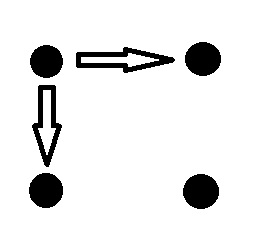
\includegraphics[width=0.5\textwidth]{22lattice}
\caption{A two by two lattice and how they interact using the Ising model}
\label{fig:22lattice}
\end{figure}
\noindent From \figref{22lattice} we see how the Ising model works on a 2x2 lattice and from this the energy is calculated. One can observe that energy is non-zero on lattices where all the objects have the same spin ($-8J$) and where the two diagonals have opposite spin from each other ($8J$). All other settings have zero energy. Knowing the energy values we can calculate the mean energy $<E>$ with our specific partition function:

$$
<E> = \frac{1}{Z}\sum^{M}_{i = 1} E_i e^{-\beta E_i}
$$
$$
 = \frac{1}{2e^{-8} + 2e^{8} + 12}\sum^{16}_{1} E_i e^{-\beta E_i}
$$
$$
 = \frac{16e^{-8}-16e^{8}}{2e^{-8} + 2e^{8} + 12} = -7.983928
$$

\noindent Now we can simply put the same energy values into our partition function:

$$
Z = e^{-\beta * -8J} + e^{-\beta * -8J} + e^{-\beta * 8J} + e^{-\beta * 8J} + 12*e^0
$$
$$
Z = 2e^{-8J\beta} + 2e^{8J\beta} + 12
$$

\noindent The magnetization is given by:

$$
M = \sum^{N}_{j = 1} s_j
$$

\noindent Unlike in the energy case, the magnetization does not depend the lattice having the same spin or that the diagonals have opposite spin. The only case where the magnetization is zero in a 2x2 lattice is when half of the objects in the lattice opposite spins. Therefore we get the magnetization values:

$$
M_i = [4 + 2 + 2 + 2 + 2 + 0 + 0 + 0 + 0 + 0 + 0 + -2 + -2 + -2 + -2 + -4]
$$

\noindent To calculate the mean magnetic moment or mean magnetization we use the equation below with our calculated magnetic moment and energy values:

$$
|M| = \frac{1}{Z}\sum^{M}_{i}M_ie^{-\beta E_i}
$$
$$
 = \frac{1}{2e^{-8} + 2e^8 + 12}\sum^{16}_{1}M_ie^{-\beta E_i}
$$
$$
 = \frac{8e^{8} + 16}{2e^{-8} + 2e^8 + 12} = 3.994643
$$



\noindent To calculate the the specific heat, one only needs to know the total number of spins of the lattice. In the 2x2 lattice case the total number of spins is 4, and remember also that $\beta J = 1$ and $k = 1$. The specific heat is then:

$$
C_V = \frac{1}{kT^2}(<E^2> - <E>^2)
$$
$$
 = \frac{1}{kT^2}(\frac{128e^{-8} - 128e^8}{2e^{-8} + 2e^8 + 12} - (\frac{16e^{-8} - 16e^8}{2e^{-8} + 2e^8 + 12})^2)
$$
$$
 = 0.128329
$$

\noindent The term $<E^2> - <E>^2$ is also called the variance of the energy and is precisely calculated just as shown above. The same variance calculation can be applied to calculating the susceptibility, but the energy terms have to be substituted for mean magnetization.
Let's calculate the variance separate from the desired equation this time:

$$
\sigma_M^2 = <M^2>-<M>^2 = \frac{1}{Z}\sum^{M}_{i = 1}M_i^2 e^{-\beta E_i} - (\frac{1}{Z}\sum^{M}_{i = 1}M_i e^{-\beta E_i})^2
$$

$$
 = \frac{32}{2e^{-8} + 2e^8 + 12}(e^{8}+1) - (\frac{8e^8 + 16}{2e^{-8} + 2e^8 + 12})^2 = 0.016004
$$

\noindent Remember that the $\beta = 1$ in the 2x2 lattice case, so the susceptibility would be the same as the variance in that case. We would usually have to calculate the susceptibility with the following equation:

$$
X = \frac{1}{k_bT}(<M^2> - <M>^2) = \frac{1}{k_bT}\sigma_M^2 = 0.010853
$$

\newpage

\begin{center}
{\LARGE\bf Results}
\end{center}

From the general equations in the method, the following analytical and numerical values were found:

\begin{table} [H]
\caption{Analytical and numerical solutions} \label{tab:table1}
\centerline{
\begin{tabular}{|c|c|c|c|}
\hline
Type & Analytical & Numerical & MC cycles needed\\
\hline
$<E>$ & -7.983928 & -7.98437 & 10 000\\
\hline
$<M>$ & 3.994643 & 3.99483 & 10 000\\
\hline
$C_V$ & 0.128329 & 0.124812 & 100 000\\
\hline
$<X>$ & 0.016004 & 0.0153613 & 100 000\\
\hline
\end{tabular}
}
\end{table}

\noindent To get good results for mean energy and mean magnetic moment took very few Monte Carlo, or MC, cycles, only about 10 000. Then the values would be off only by a factor of about $10^{-3}$. The susceptibility and the specific heat took more MC cycles and correct results started showing around $10^{5}$ for susceptibility and specific heat. For $10^4$ both the specific heat and susceptibility were unstable.

\begin{figure}[H]
\centerline{
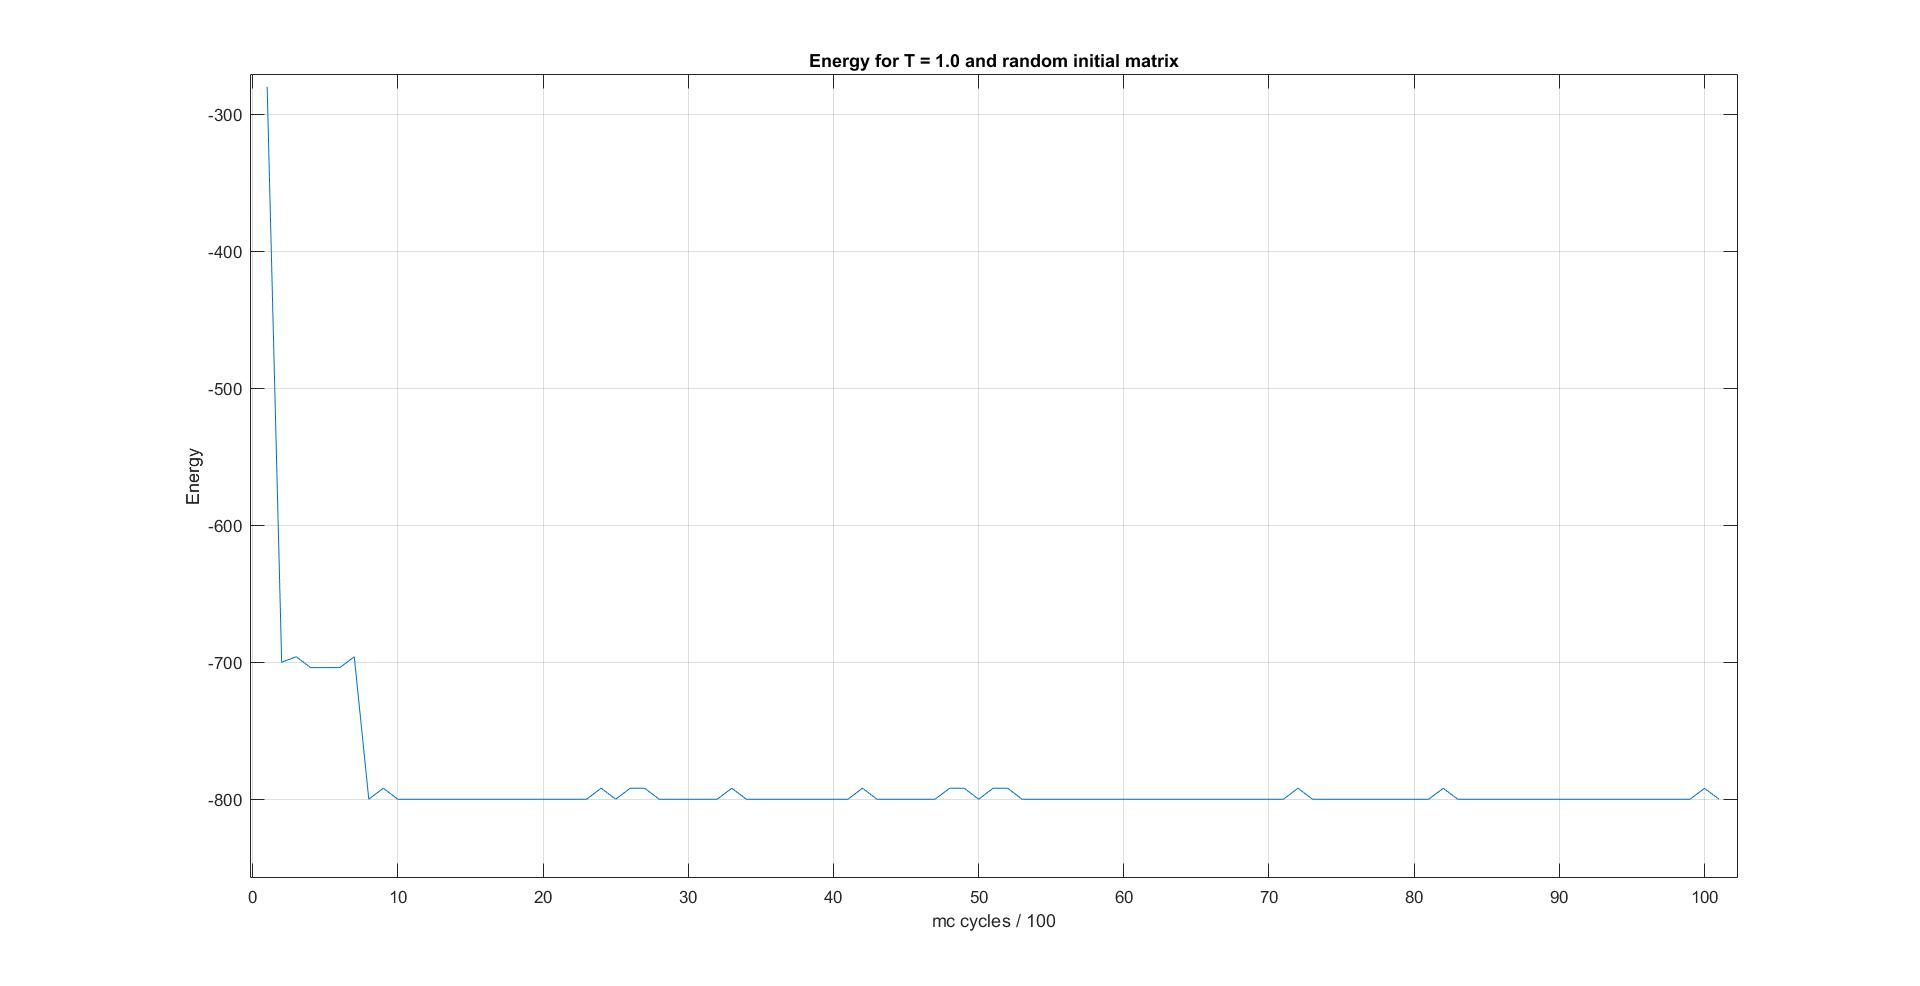
\includegraphics[width=0.7\textwidth]{energyT1random}
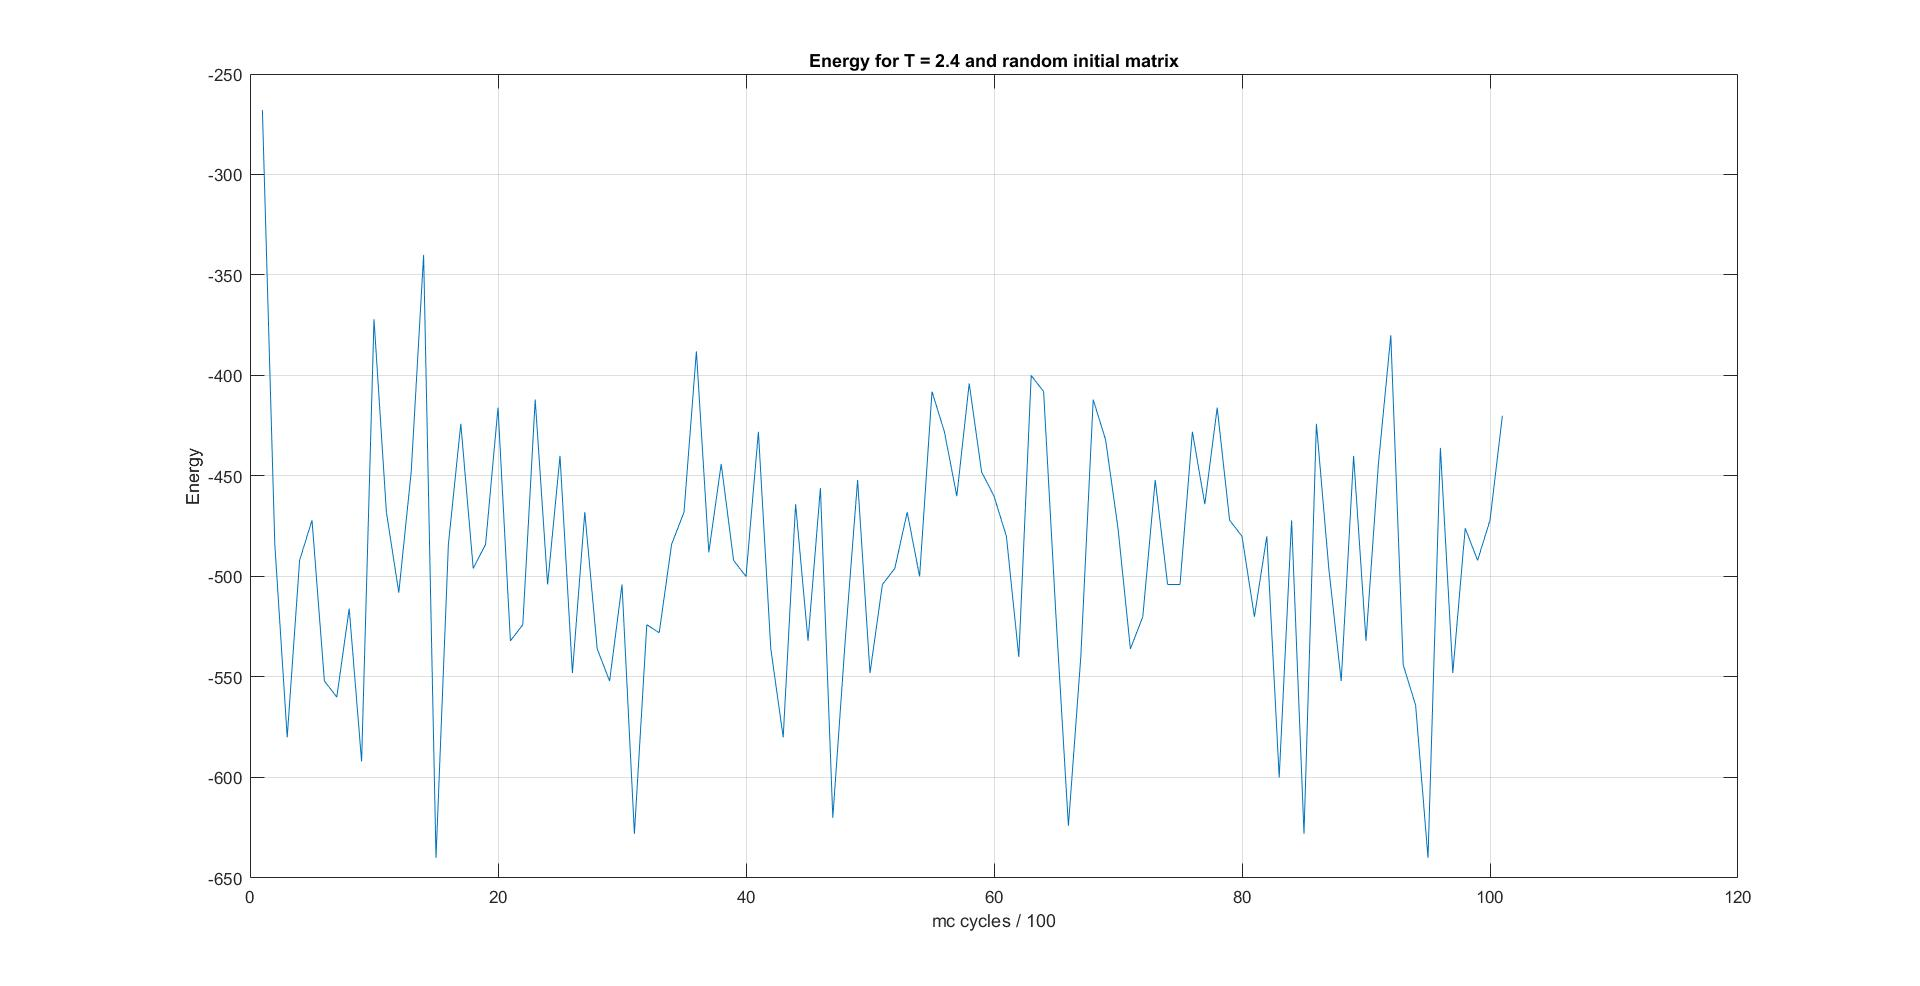
\includegraphics[width=0.7\textwidth]{energyT24random}
}
\caption{Energy versus Monte Carlo cycles for T = 1.0 and T = 2.4 with a random initial matrix}
\label{fig:energyrandom}
\end{figure}

\begin{figure}[H]
\centerline{
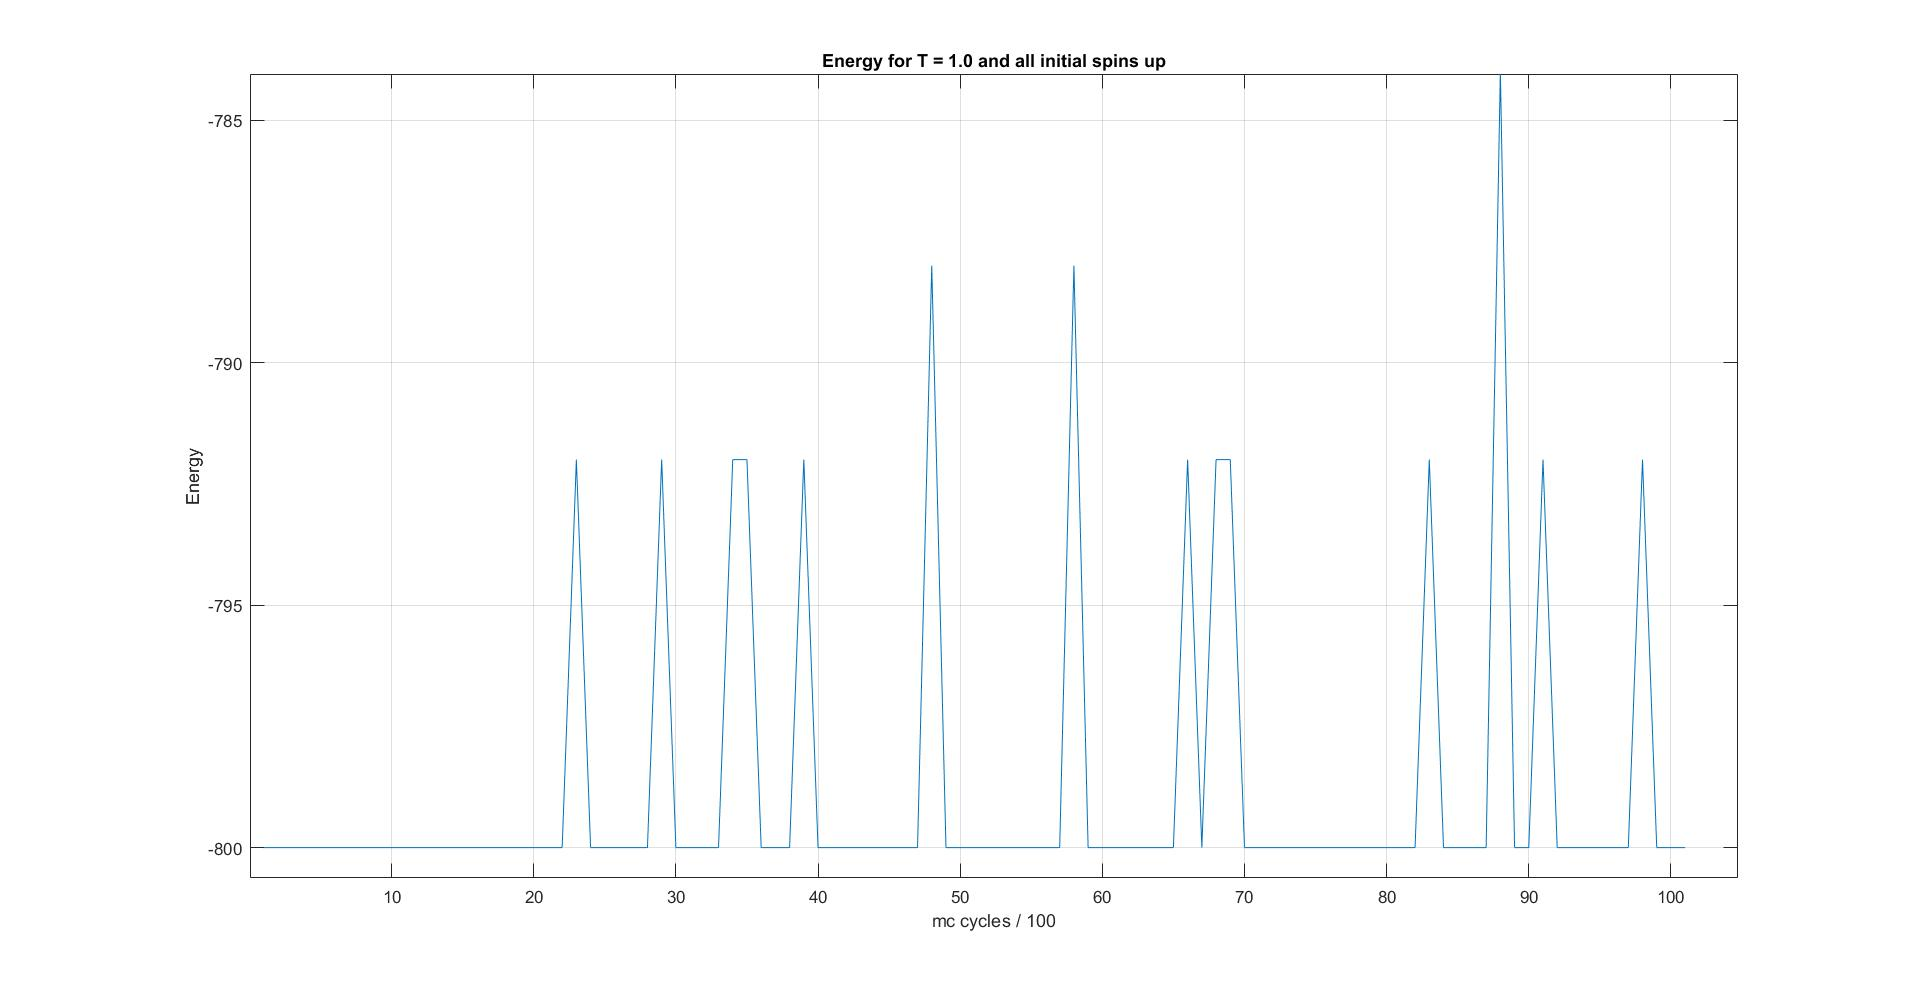
\includegraphics[width=0.7\textwidth]{energyT1upspin}
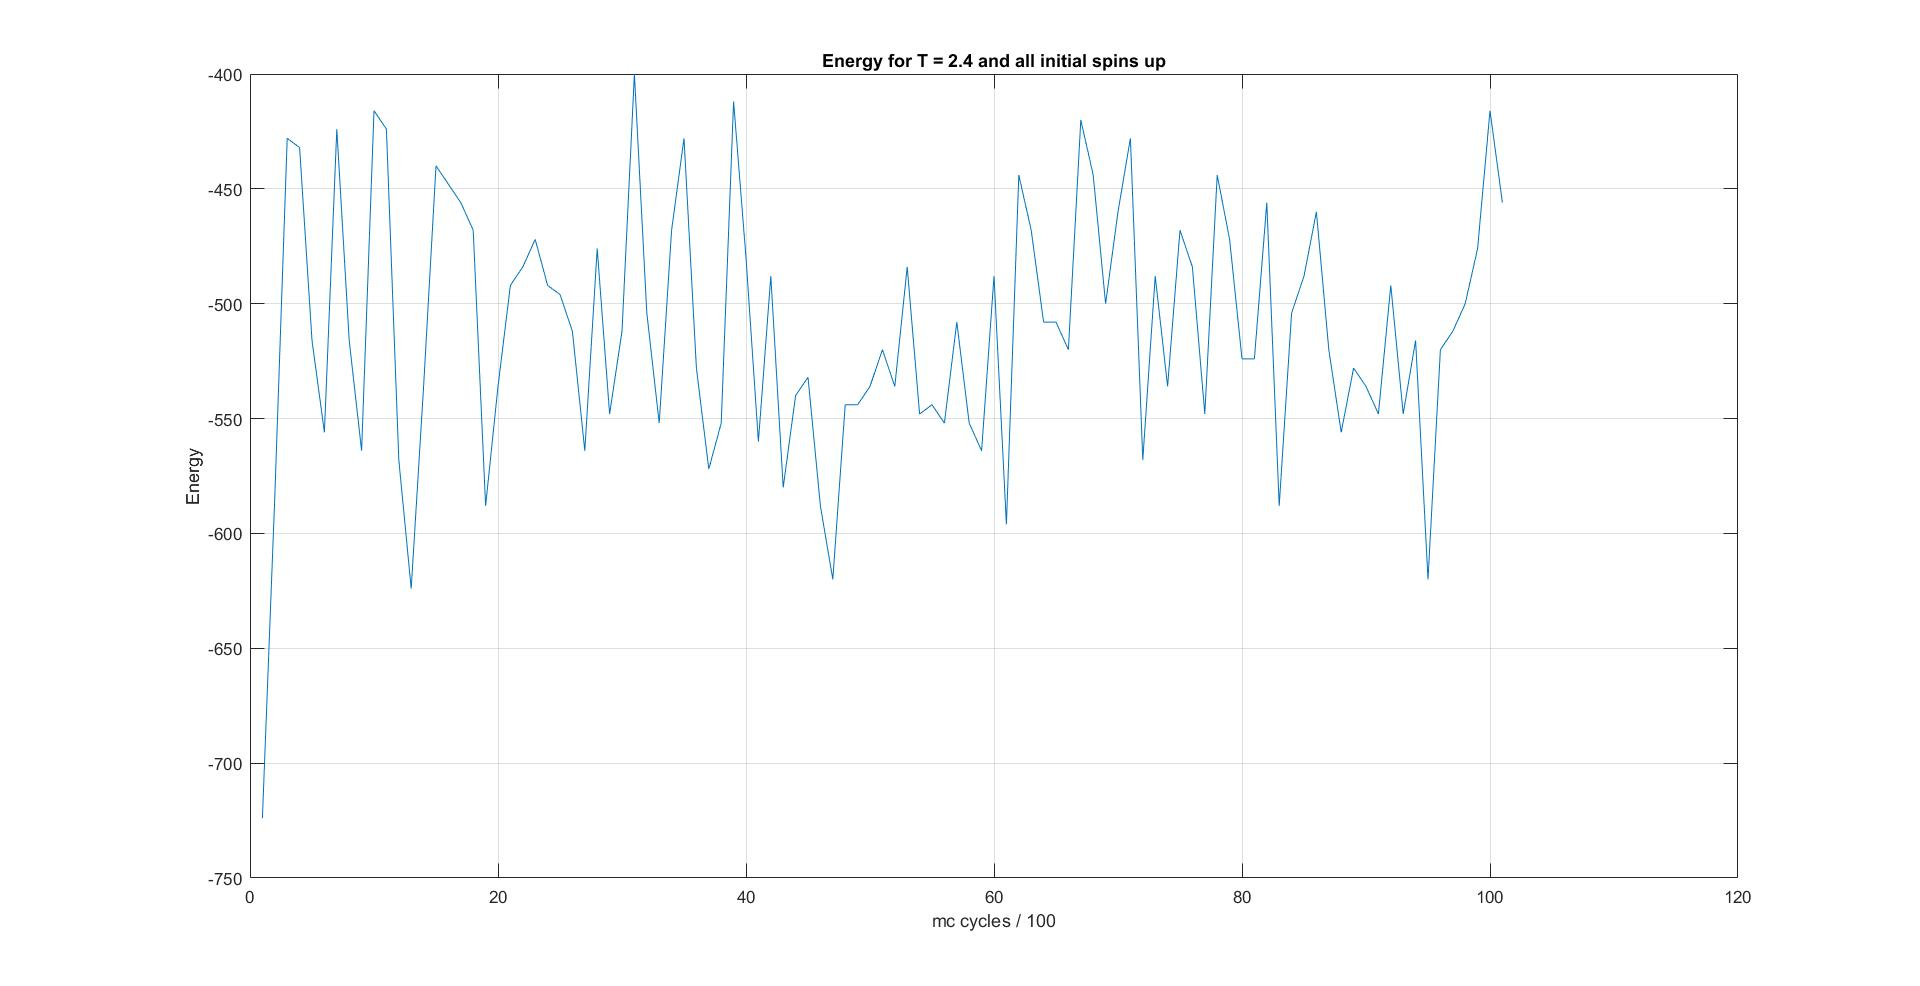
\includegraphics[width=0.7\textwidth]{energyT24upspin}
}
\caption{Energy versus Monte Carlo cycles for T = 1.0 and T = 2.4 with initial spin upwards}
\label{fig:energyupspin}
\end{figure}

\begin{figure}[H]
\centerline{
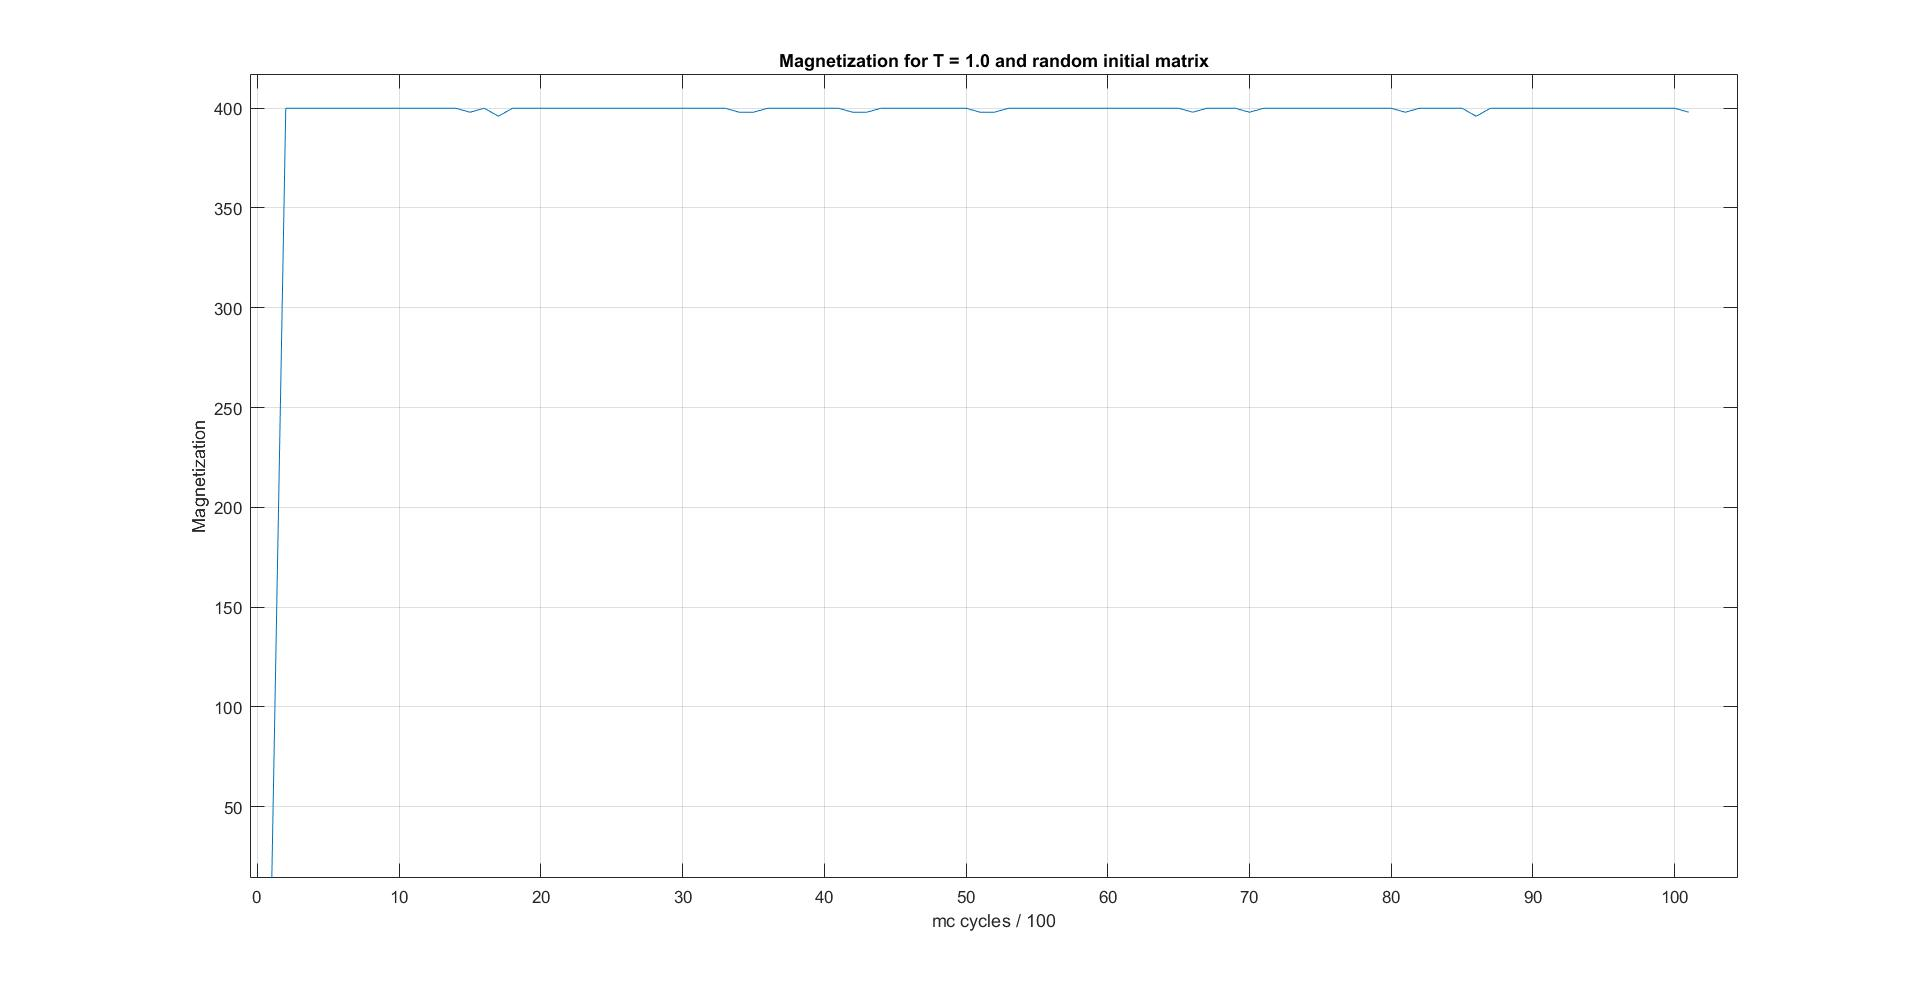
\includegraphics[width=0.7\textwidth]{magnetizationT1random}
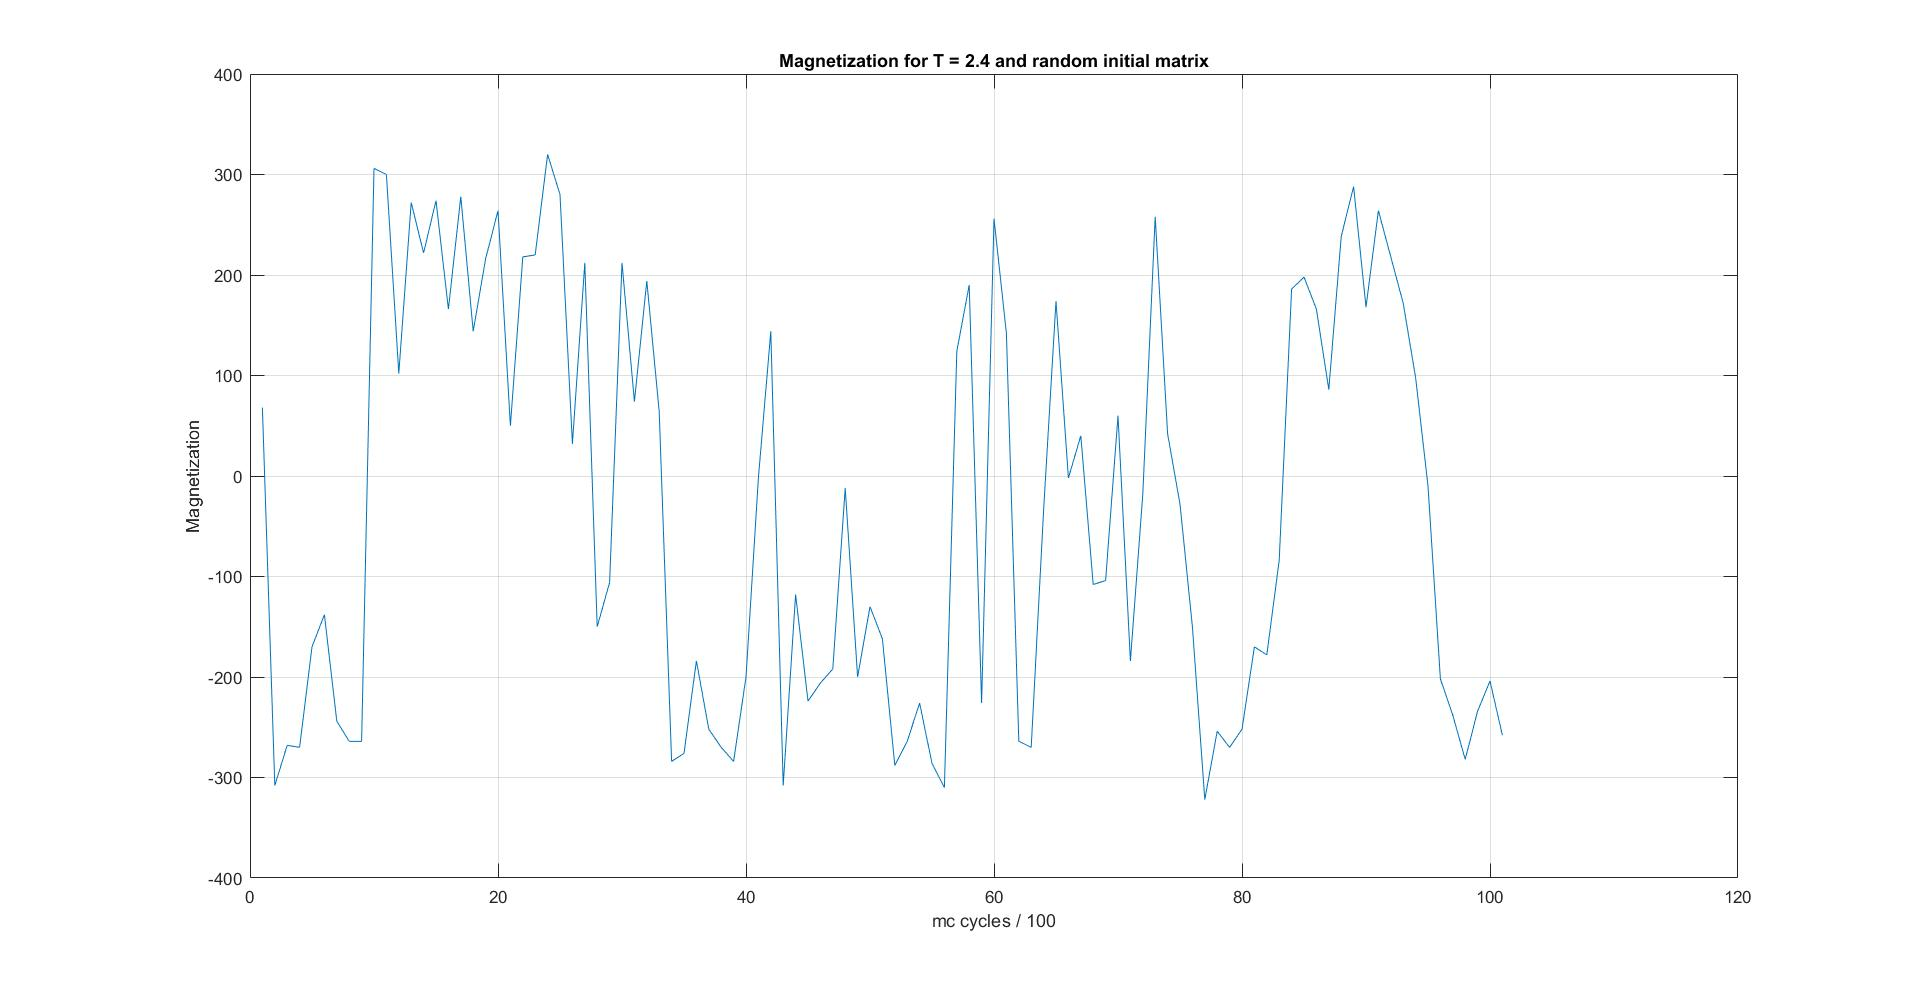
\includegraphics[width=0.7\textwidth]{magnetizationT24random}
}
\caption{Magnetization versus Monte Carlo cycles for T = 1.0 and T = 2.4 with a random initial matrix}
\label{fig:magneticrandom}
\end{figure}

\begin{figure}[H]
\centerline{
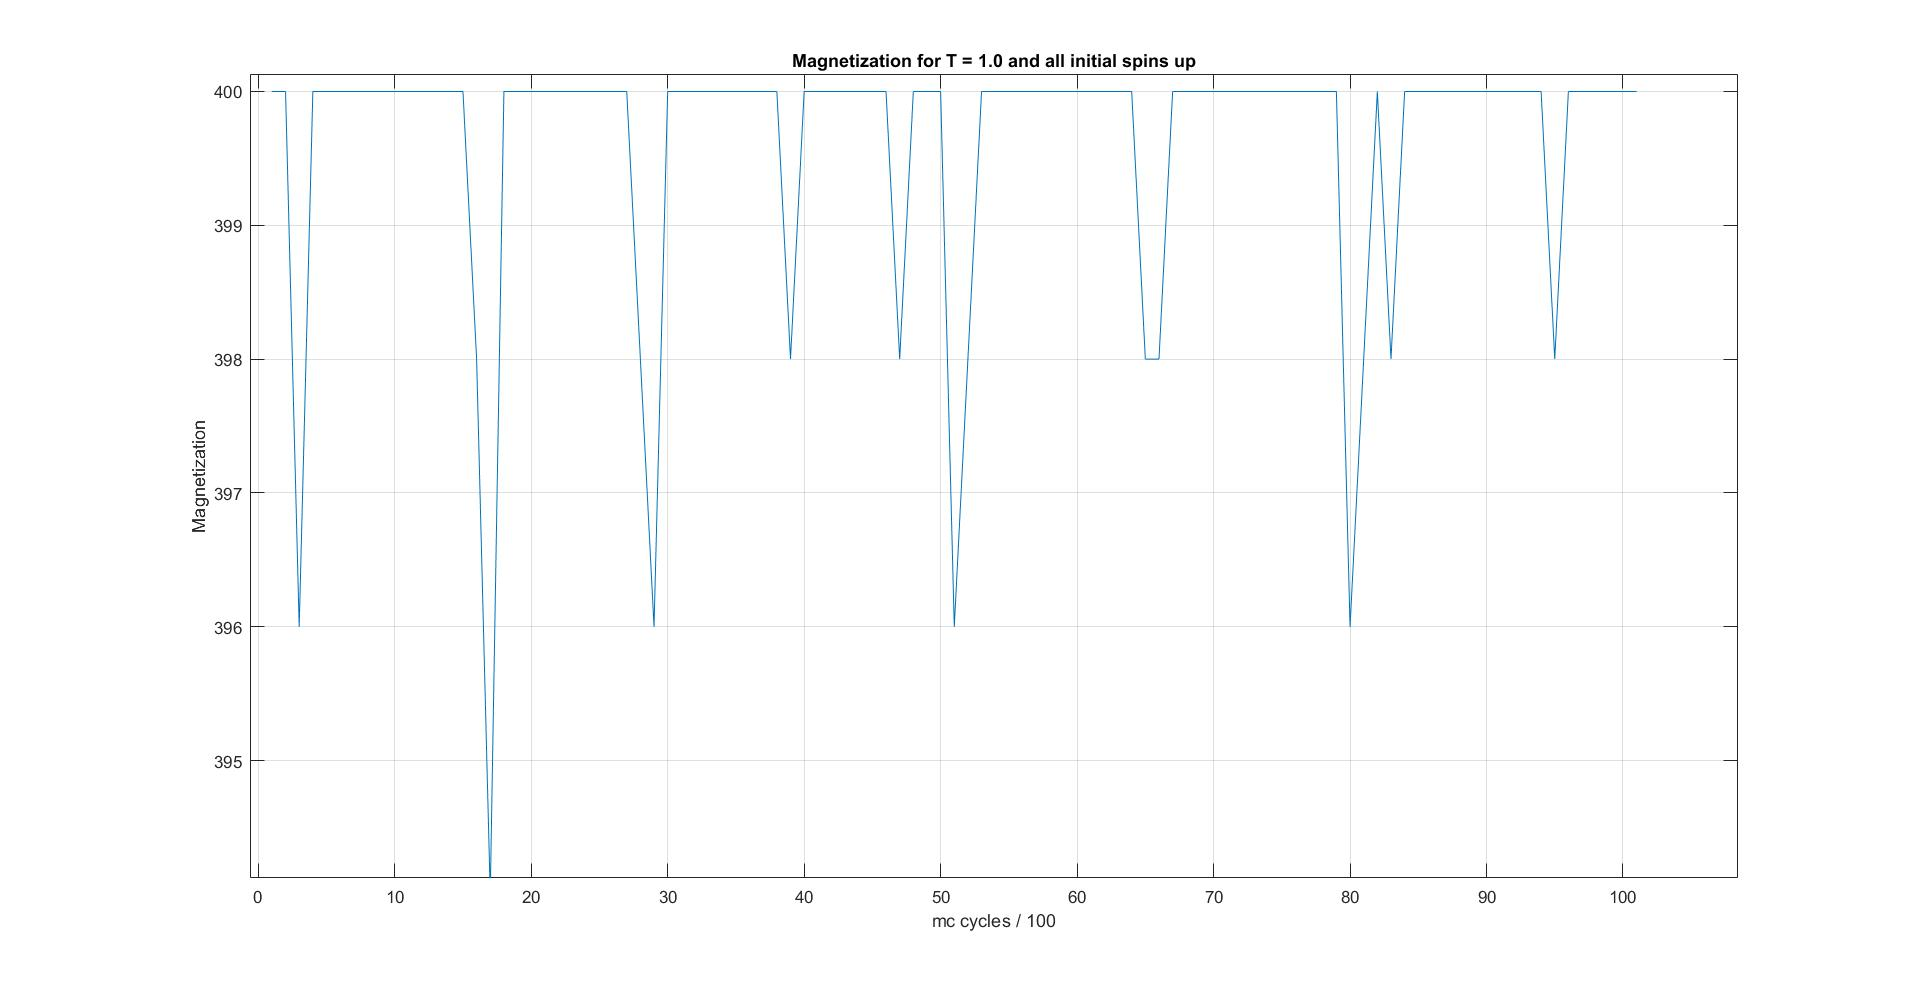
\includegraphics[width=0.7\textwidth]{magnetizationT1upspin}
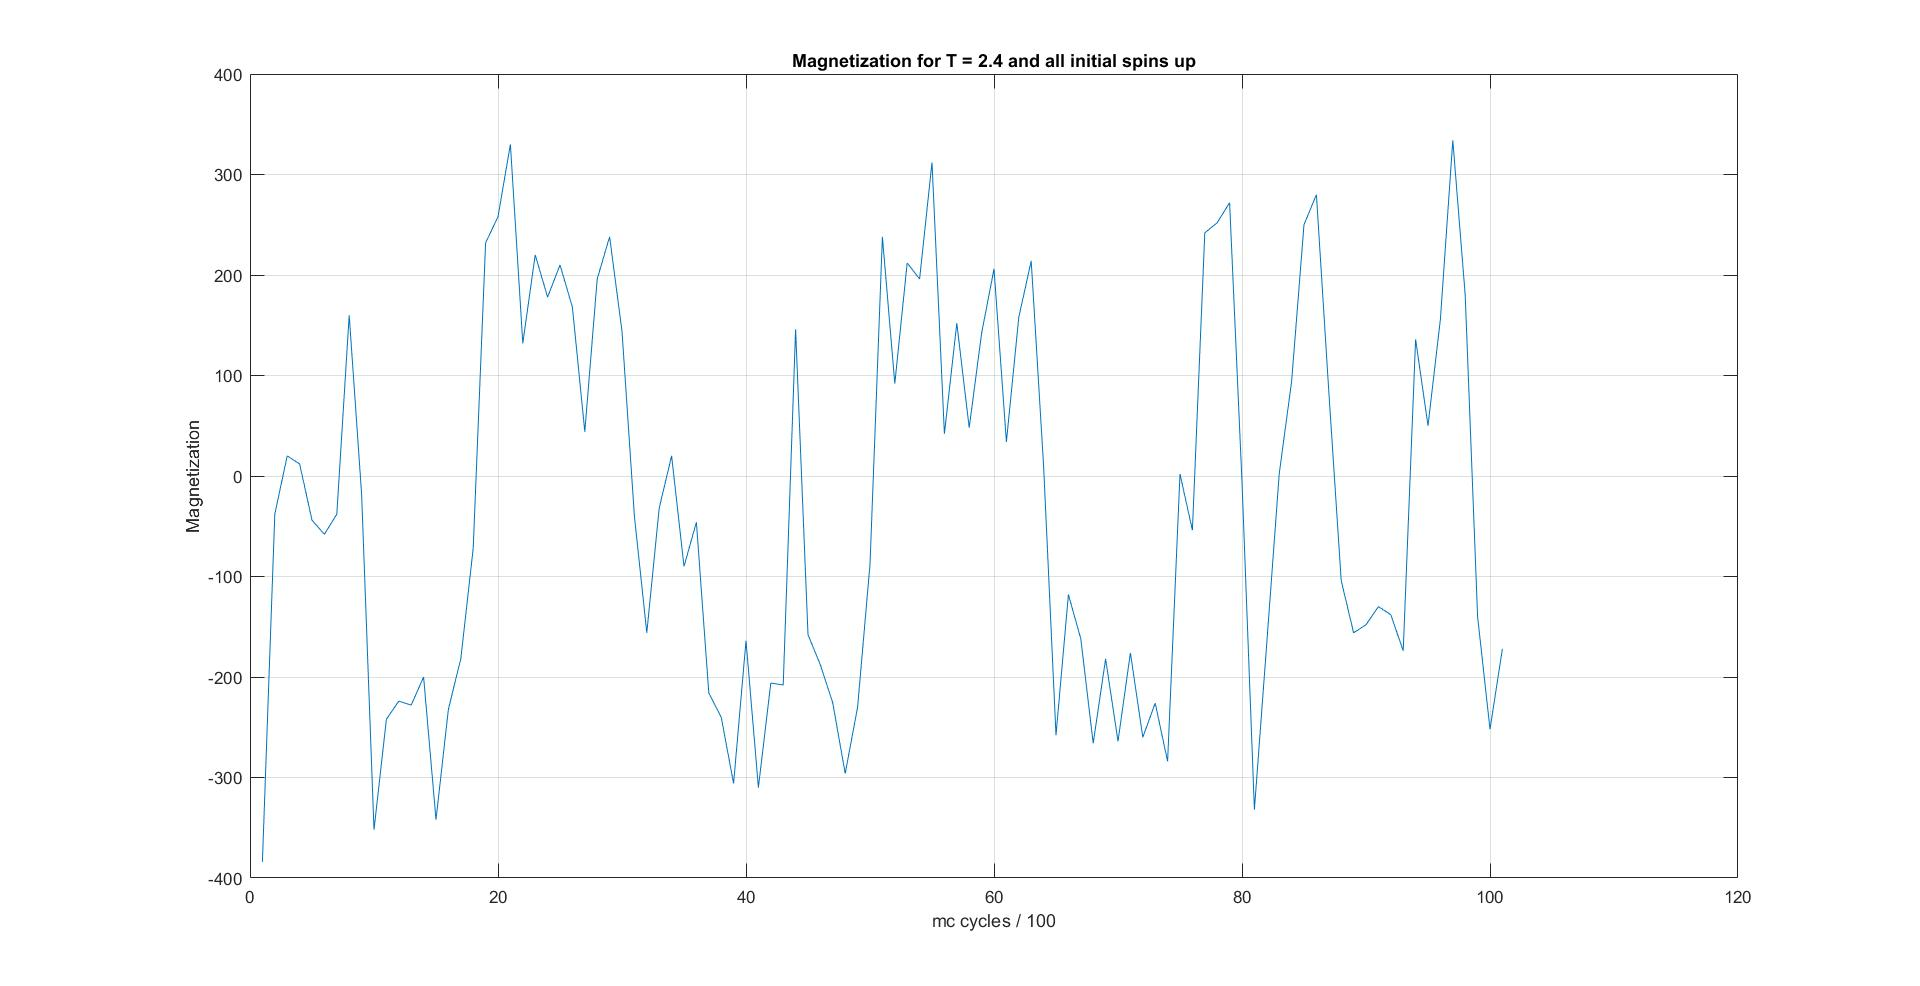
\includegraphics[width=0.7\textwidth]{magnetizationT24upspin}
}
\caption{Magnetization versus Monte Carlo cycles for T = 1.0 and T = 2.4 with initial spin upwards}
\label{fig:magneticupspin}
\end{figure}

\noindent We can see from \figref{energyrandom}, \figref{energyupspin}, \figref{magneticrandom} and \figref{magneticupspin} that the mean energy and magnetization quickly approaches it's equilibrium state when the temperature equals 1. There are of coarse fluctuations after the mean energy and magnetization has reached it's equilibrium state, but the value tends to jump back to to the equilibrium state. Another observation is that the mean energy and magnetization value are more unstable if one starts with an initial matrix where all the spins are oriented upwards. The values become even more unstable when the temperature is increased to 2.4, and also the value of the equilibrium state is changed. 

\begin{table} [H]
\caption{EQ values for energy} \label{tab:table2}
\centerline{
\begin{tabular}{|c|c|c|c|}
\hline
Orientation & Temperature & EQ state & max MC cycles needed\\
\hline
Random & 1.0 & -790.581 & 600\\
\hline
Random & 2.4 & -496.494 & 1000\\
\hline
Upwards & 1.0 & -798.96 & 1\\
\hline
Upwards & 2.4 & -493.996 & 300\\
\hline
\end{tabular}
}
\end{table}

\begin{table}[H]
\caption{EQ values for magnetization} \label{tab:table3}
\centerline{
\begin{tabular}{|c|c|c|c|}
\hline
Orientation & Temperature & EQ state & max MC cycles needed\\
\hline
Random & 1.0 & 398.762 & ???\\
\hline
Random & 2.4 & 165.209 & ???\\
\hline
Upwards & 1.0 & 399.732 & 1\\
\hline
Upwards & 2.4 & 176.087 & ???\\
\hline
\end{tabular}
}
\end{table}

\begin{figure}[H]
\centerline{
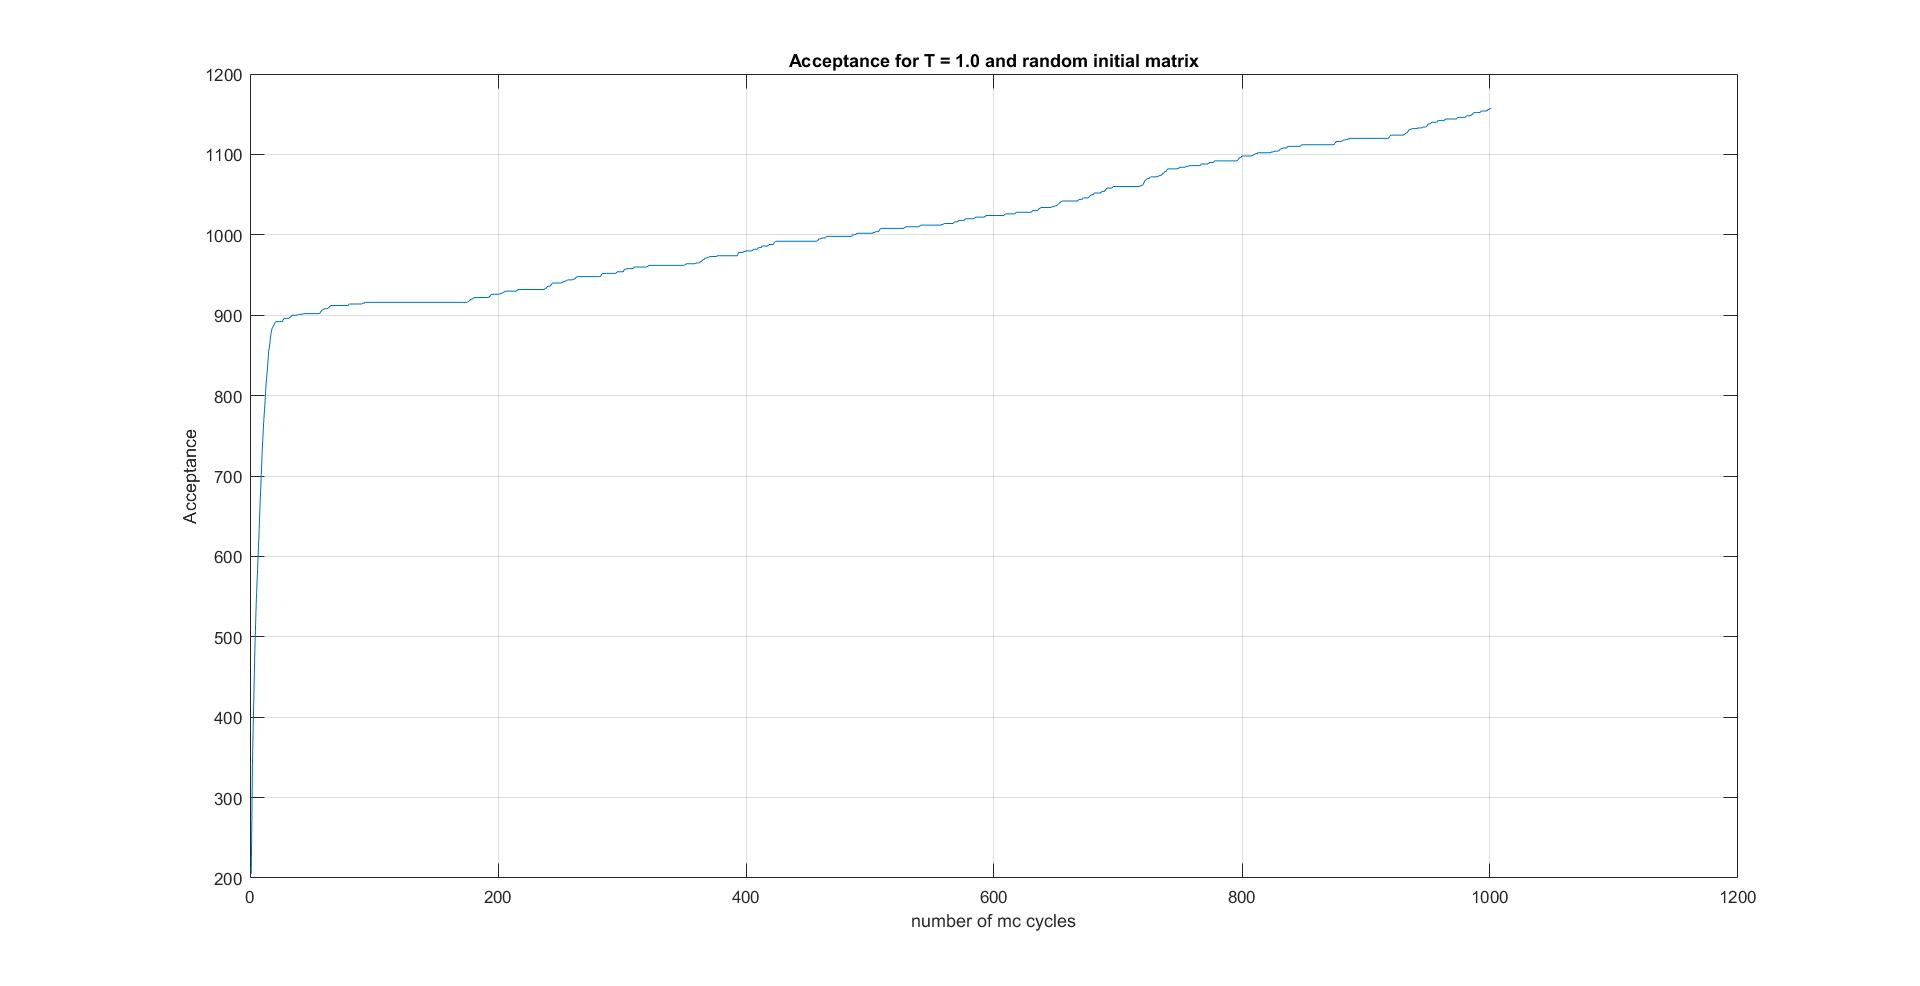
\includegraphics[width=0.7\textwidth]{acceptanceMCT1random}
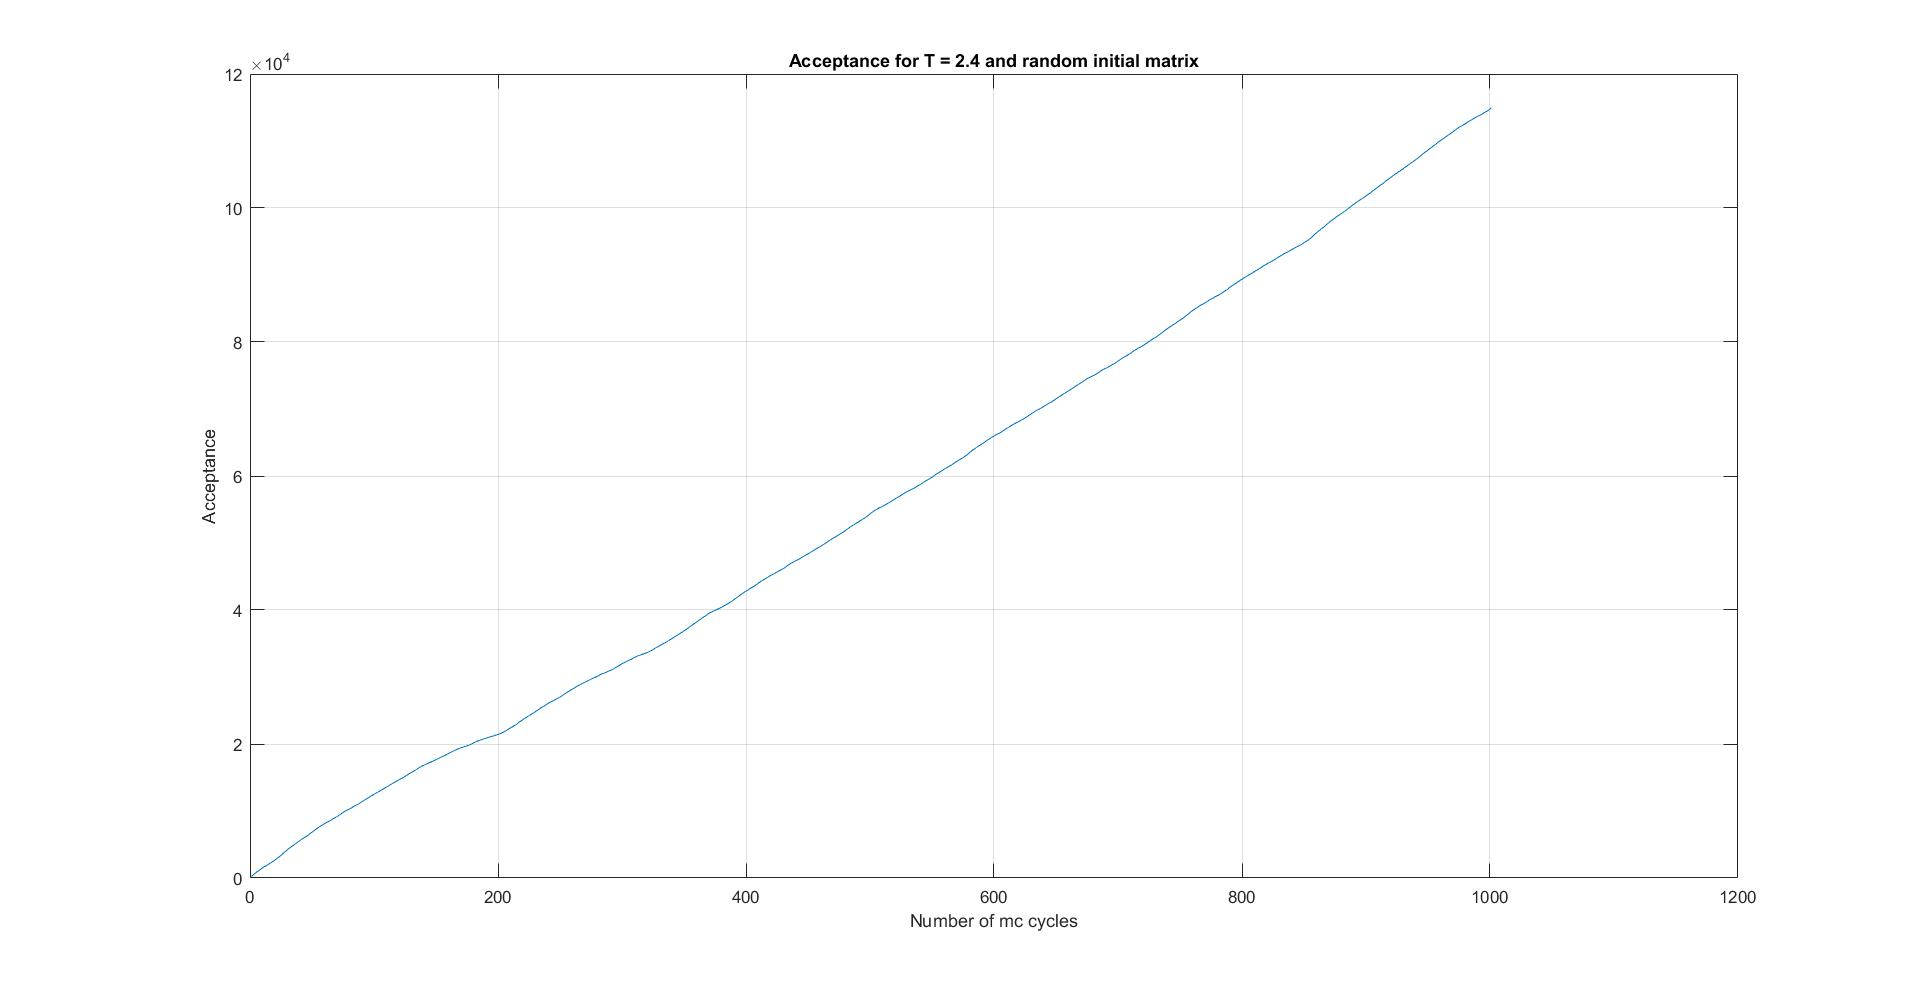
\includegraphics[width=0.7\textwidth]{acceptanceMCT24random}
}
\caption{Acceptance versus Monte Carlo cycles for T = 1.0 and T = 2.4 with a random initial matrix}
\label{fig:acceptancerandom}
\end{figure}

\begin{figure}[H]
\centerline{
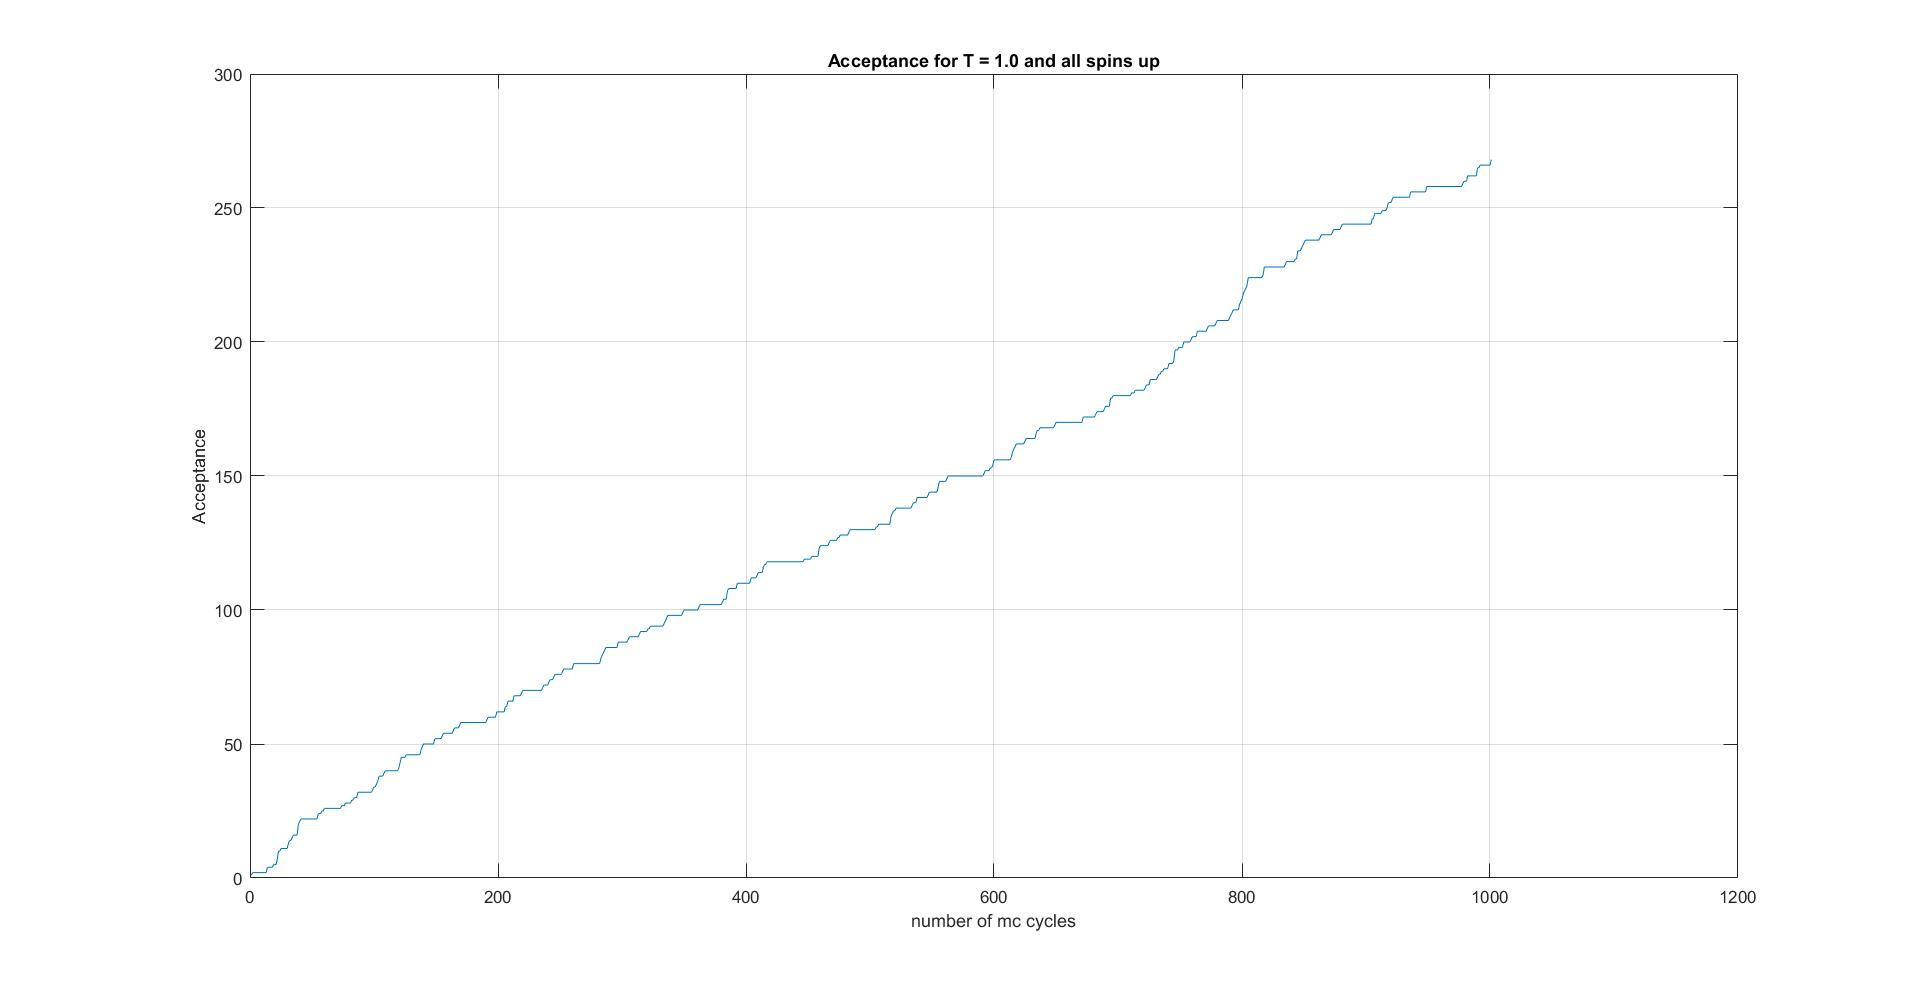
\includegraphics[width=0.7\textwidth]{acceptanceMCT1upspin}
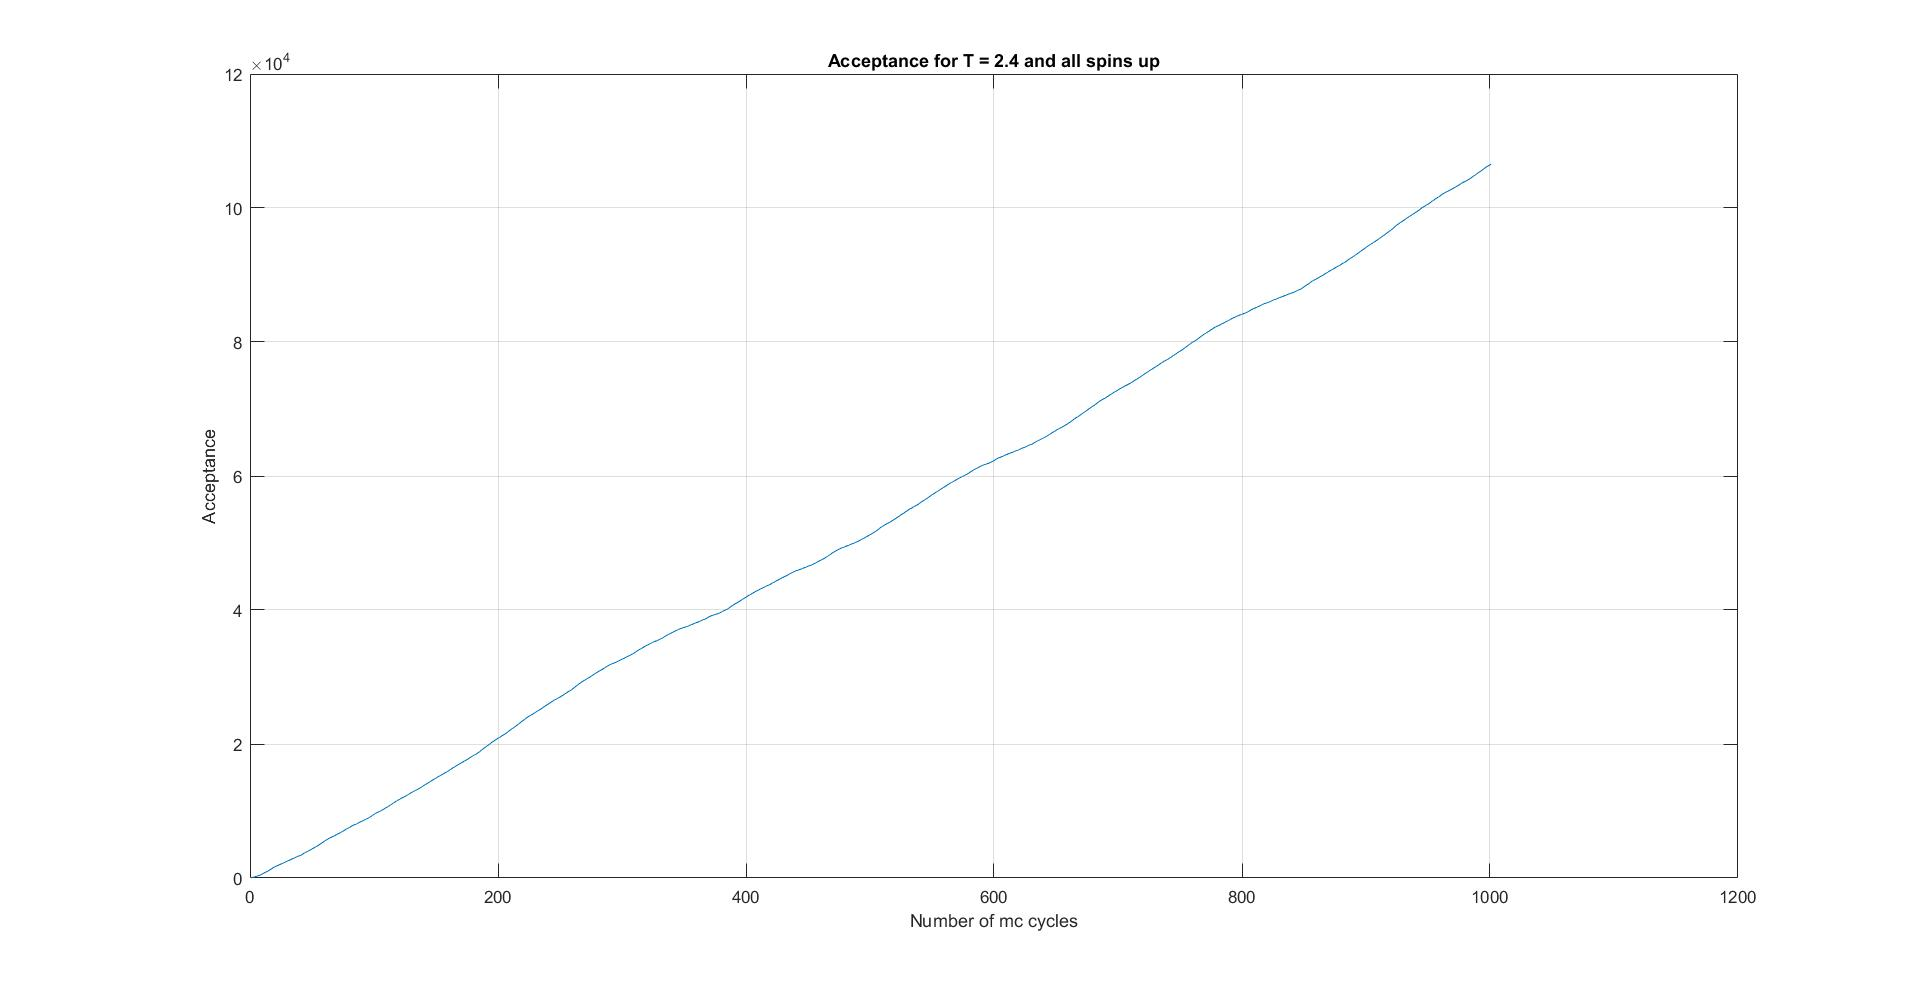
\includegraphics[width=0.7\textwidth]{acceptanceMCT24upspin}
}
\caption{Acceptance versus Monte Carlo cycles for T = 1.0 and T = 2.4 with initial spin upwards}
\label{fig:acceptanceupspin}
\end{figure}

\begin{figure}[H]
\centerline{
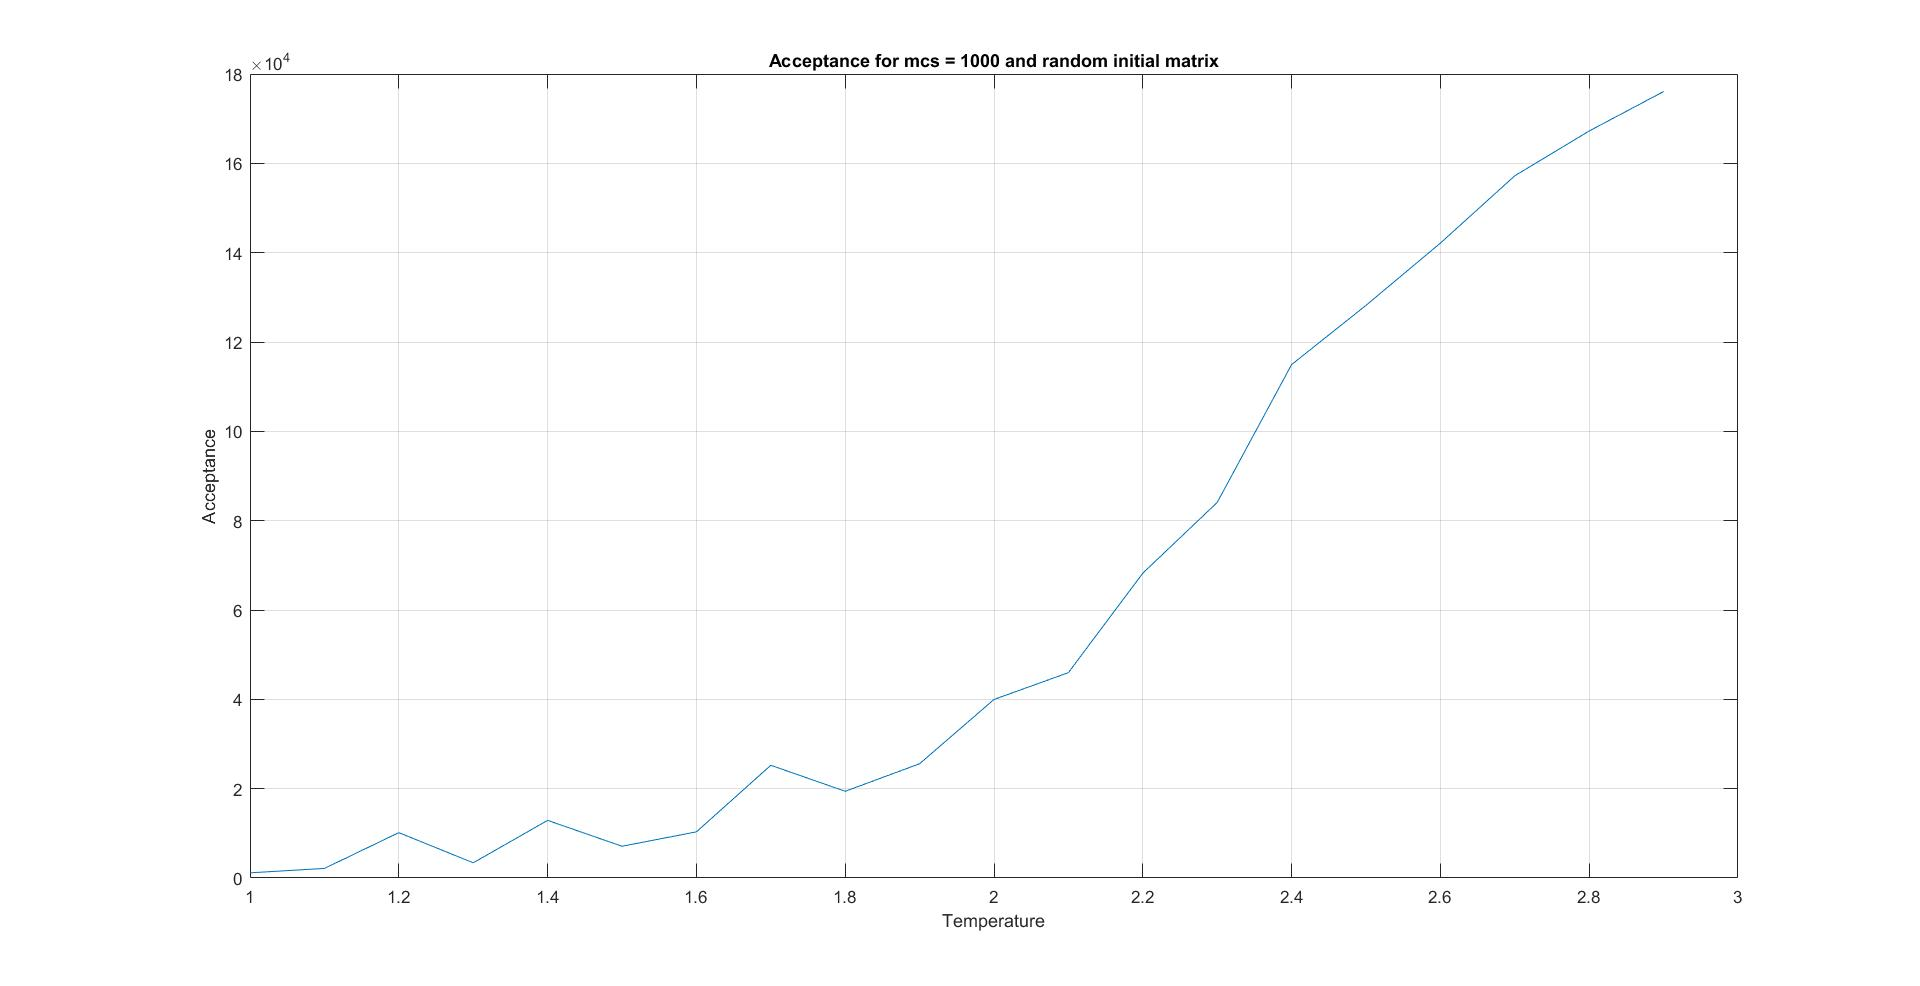
\includegraphics[width=0.7\textwidth]{acceptanceVStrandom}
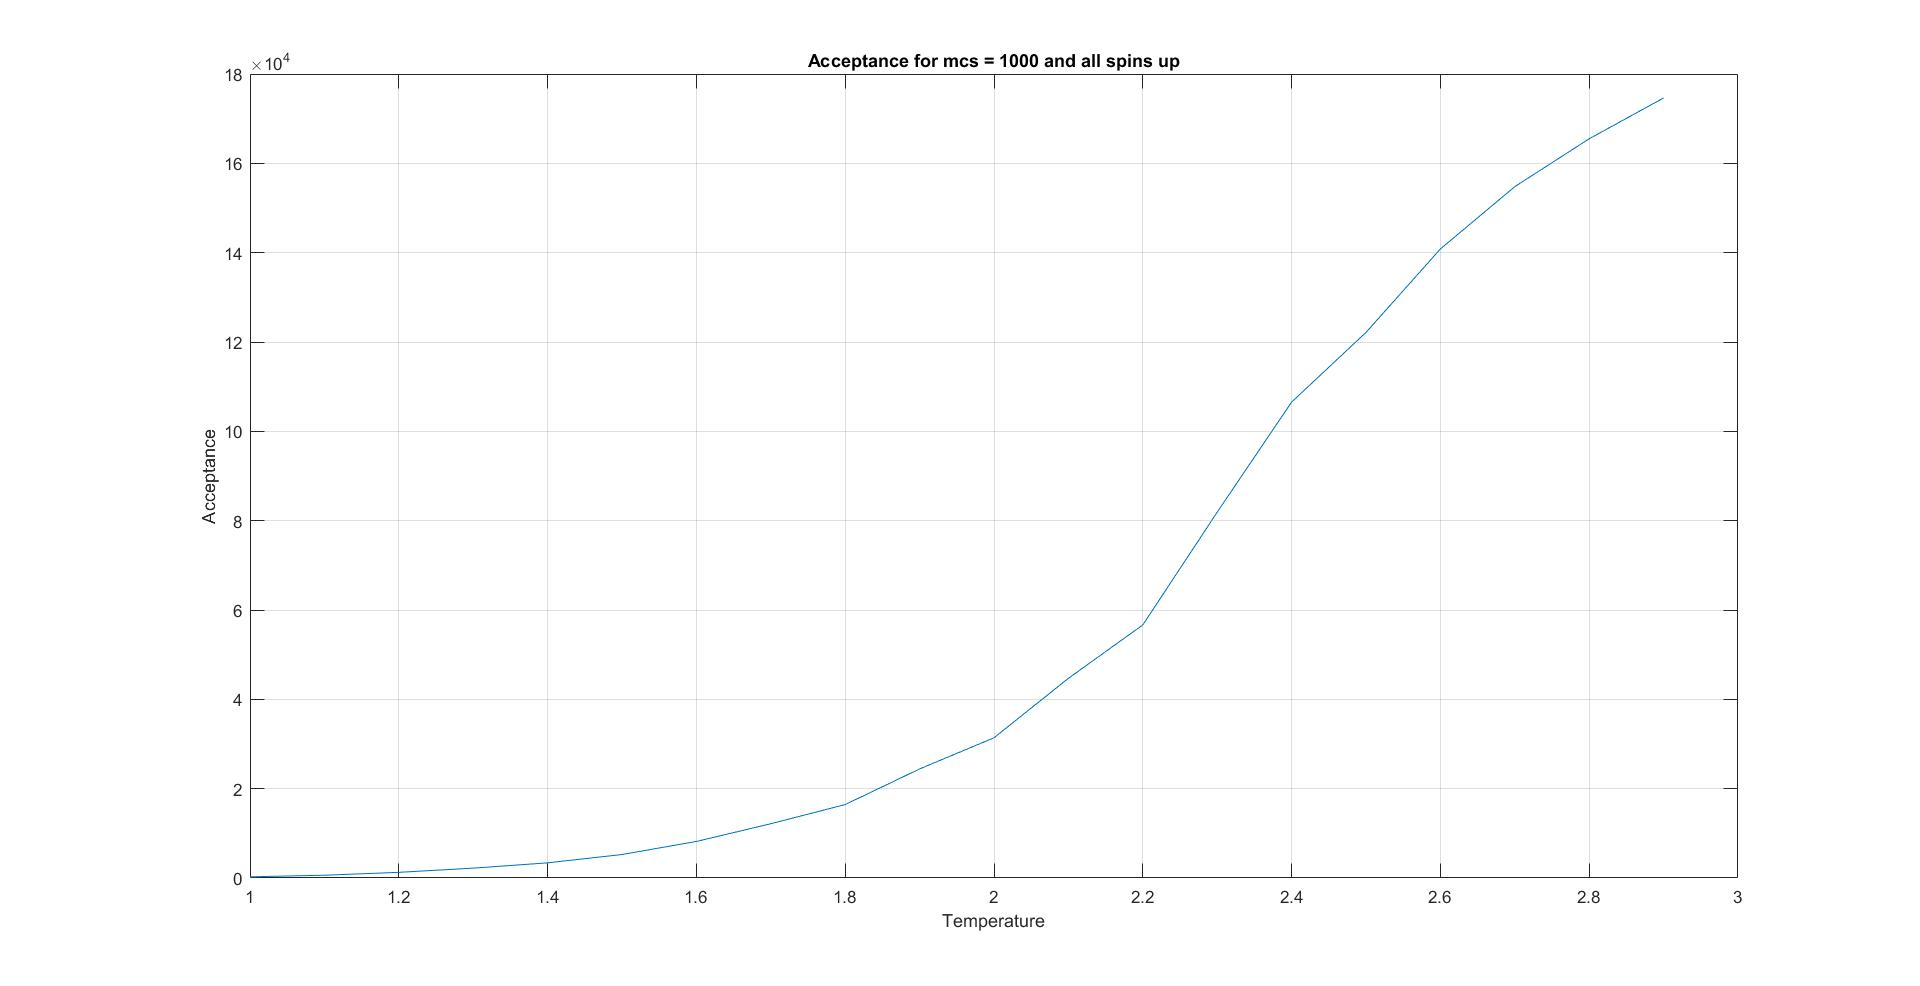
\includegraphics[width=0.7\textwidth]{acceptanceVStupspin}
}
\caption{Acceptance versus temperature for a random initial matrix and with initial spin upwards}
\label{fig:acceptancetemp}
\end{figure}

\noindent Acceptance is apparently also dependent on both temperature and the initial state of the spins. From figure \figref{acceptancerandom} one can observe that with higher temperature the number of accepted values increase by a factor of $10$. For $T = 1.0$, one can also observe that the acceptance spikes for few Monte Carlo cycles. 
\\
If the initial spins are all positive like in \figref{acceptanceupspin}, the acceptance becomes more linear. The line for $T = 1.0$ is more squiggly than the straighter line for $T = 2.4$. The ladder does not spike for few Monte Carlo cycles in this case.
\\
From \figref{acceptancetemp}, one can observe that the curves are not linear. The curve based on a randomly generated initial matrix is uneven at low temperatures, but smooths out when $T$ increases. When the initial matrix only consist positive spins, the curve is smooth throughout. These two plots are plotted to a maximum temperature of $3.0$, so one would have an idea of how the acceptance would evolve after $T = 2.4$. 



\end{document}